\clearpage % Start a new page
\lhead{\emph{Predicción de series temporales}}
\chapter{Predicción de series temporales}
\label{sec:Prediccion de series temporales}

Este trabajo se centra en la predicción del comportamiento futuro de estas series temporales mediante el uso de técnicas estadísticas y de aprendizaje automático. A continuación, se proporciona una base teórica, que incluye una introducción a las series temporales, una explicación del modelo ARIMA y sus componentes, y, por último, se aborda el uso de redes neuronales recurrentes para realizar pronósticos más avanzados.

\section{Series Temporales}

Una serie temporal es una secuencia de observaciones orientadas en el tiempo o cronológicas sobre una variable de interés \cite{kulahci2015introduction}. Este tipo de datos permite examinar cómo varían las variables asociadas a lo largo del tiempo. Los valores consecutivos en una serie temporal suelen estar altamente correlacionados, lo que refleja la dependencia entre las observaciones a lo largo del tiempo. Así, el valor en un momento determinado no es independiente, sino que depende de los valores anteriores en la secuencia, lo que facilita la identificación de patrones y tendencias a lo largo del tiempo. Si se utilizan los valores de estos instantes de tiempo como características independientes, se pierde información clave sobre las relaciones entre los valores de dichos instantes \cite{aggarwal2018neural}. 


Las series temporales pueden presentar diversas características, como una tendencia, estacionalidad, o incluso ambas simultáneamente. Asimismo, pueden clasificarse como estacionarias o no estacionarias, dependiendo de si sus propiedades estadísticas, como la media y la varianza, permanecen constantes a lo largo del tiempo. Es importante destacar que los conceptos de estacionalidad y estacionariedad en una serie temporal son diferentes. A continuación, se proporcionará una explicación más detallada para clarificar estos términos; sin embargo, por el momento, es útil señalar que la estacionalidad se refiere al término en inglés \textit{seasonality}, mientras que la estacionariedad corresponde al término \textit{stationarity}.

La media en una serie temporal que se define como la esperanza matemática del valor de la variable en un instante determinado. Representa el promedio esperado del proceso y describe el nivel central en torno al cual fluctúan las observaciones. En el caso de una serie estacionaria, esta media permanece constante a lo largo del tiempo, lo cual es una propiedad clave para el análisis estadístico y la modelación del proceso \cite{box2015time}.


La varianza en una serie temporal que expresa el grado de dispersión de los valores con respecto a su media. Es una medida fundamental de la variabilidad del proceso. En particular, la varianza se interpreta como un caso especial de la autocovarianza cuando se analiza un mismo punto en el tiempo. Una serie estacionaria requiere que la varianza permanezca constante en el tiempo. Si esta cambia, la serie se considera no estacionaria, lo que afecta la elección de los modelos de predicción adecuados \cite{box2015time}.


La tendencia se refiere al comportamiento general de la serie temporal, donde se observa un incremento o decrecimiento sostenido a lo largo de un período prolongado de tiempo.

La estacionalidad se refiere a patrones que se repiten de manera regular en intervalos de tiempo más cortos que un año. Estos ciclos recurrentes presentan una variación consistente y siempre tienen un período fijo.

Una serie temporal estacionaria es aquella cuyas propiedades estadísticas son independientes del momento en que se observa la serie. En otras palabras, en una serie temporal estacionaria, aspectos fundamentales como la media, la varianza y la distribución de los datos se mantienen constantes a lo largo del tiempo. Una serie que presenta estacionalidad no es estacionaria en términos estrictos, a menos que dichos efectos se eliminen mediante técnicas como la diferenciación estacional. Esta distinción es crucial para seleccionar modelos adecuados y garantizar la validez del análisis \cite{hyndman}, \cite{shumway2011time}.


En el modelado de series temporales, es fundamental introducir los conceptos de ventana de tiempo y horizonte de pronóstico. La ventana de tiempo se refiere al número de valores u observaciones en periodos anteriores que se consideran útiles para realizar el pronóstico, partiendo del supuesto de que los eventos pasados pueden influir en el futuro o proporcionar información relevante. Por otro lado, el horizonte de pronóstico se refiere a la cantidad de periodos futuros que se pretende predecir en el contexto del modelado de series temporales.

El ruido blanco es un concepto clave en el análisis de series temporales, que se refiere a un tipo de proceso estocástico donde no existe una estructura discernible ni patrones predecibles en los datos. Es decir, cada observación es completamente independiente de las demás y no está influenciada por eventos pasados. Habitualmente, se denota con la letra $\epsilon$ (épsilon).

Por último, es relevante mencionar que los pronósticos pueden ser de corto, mediano o largo plazo. Los pronósticos a corto plazo abarcan periodos de días, semanas o meses; los de mediano plazo comprenden entre 1 y 2 años; y los pronósticos que superan este rango se consideran de largo plazo \cite{kulahci2015introduction}


\section{Técnicas Estadísticas}

Las técnicas estadísticas clásicas para la predicción de series temporales, como el modelo \textit{ARIMA} (Autoregressive Integrated Moving Average), se han utilizado ampliamente para modelar el comportamiento de una variable a lo largo del tiempo, analizando patrones históricos para generar pronósticos. ARIMA es una técnica estadística clásica ampliamente utilizada para el modelado de series temporales \cite{hyndman}. Combina enfoques como la autorregresión, la diferenciación y las medias móviles, lo que permite capturar la dinámica subyacente en los datos.

En el modelo ARIMA, se identifican tres parámetros clave: \(p\), \(d\) y \(q\). El parámetro \(p\) representa el número de observaciones pasadas utilizadas para predecir el valor actual de la serie, lo que corresponde a la componente de autorregresión. El parámetro \(d\) indica cuántas veces se debe diferenciar la serie temporal para eliminar tendencias y hacerla estacionaria, conocido como integración. Finalmente, \(q\) se refiere al número de errores pasados que ayudan a ajustar las predicciones, lo que constituye la parte de media móvil del modelo.

En esta sección, se utilizará la serie temporal genérica \(y_0, y_1, \dots, y_{t-2}, y_{t-1}, y_t\), donde \(y_0\) es el primer valor registrado en la serie, mientras que \(y_t\) representa el valor más reciente.

\subsection{Modelado con Auto-regresión}

La autorregresión es un enfoque de pronóstico de series temporales que depende únicamente de los valores anteriores de una serie temporal, esta técnica asume que las observaciones futuras en el siguiente punto temporal están relacionadas con los valores en puntos temporales anteriores a través de una relación lineal. Así, un modelo autorregresivo de orden \( p \) se puede escribir como \eqref{eq:autoregression} donde \( \epsilon_t \) es ruido blanco. Esto es similar a una regresión múltiple, pero con valores rezagados de \( y_t \) como predictores. Nos referimos a esto como un modelo AR(\( p \)), un modelo autorregresivo de orden \( p \). \cite{hyndman}.

\begin{equation}
y_t = \delta + \phi_1 y_{t-1} + \phi_2 y_{t-2} + \ldots + \phi_p y_{t-p} + \epsilon
\label{eq:autoregression}
\end{equation}

La ecuación \(\eqref{eq:autoregression}\) describe un modelo autorregresivo de orden \(p\), donde cada componente tiene un papel específico en la predicción del valor actual de la serie temporal \(y_t\).

En primer lugar, \(y_t\) representa el valor actual de la serie temporal en el instante \(t\). Es el objetivo de la predicción y depende de los valores pasados de la serie y de un componente de error. Este valor es crucial porque refleja el fenómeno que se está modelando, ya sea la temperatura, los precios de acciones o cualquier otra variable de interés que cambie con el tiempo.

El término \(\delta\) es una constante que actúa como el **intercepto** del modelo. Representa el nivel base de la serie temporal, el cual se suma a los demás términos. Él interceptó proporciona un ajuste general que captura cualquier sesgo constante en los datos, asegurando que el modelo pueda reflejar adecuadamente el comportamiento central de la serie, incluso cuando los valores pasados no contribuyen.

Los coeficientes \(\phi_1, \phi_2, \ldots, \phi_p\) son los parámetros del modelo que indican la influencia de los valores rezagados de la serie temporal sobre el valor actual \(y_t\). Cada coeficiente se asocia con un valor de la serie en un período anterior: \(\phi_1\) está relacionado con el valor inmediatamente anterior \(y_{t-1}\), \(\phi_2\) con el valor dos períodos atrás \(y_{t-2}\), y así sucesivamente hasta \(y_{t-p}\), que representa el valor \(p\) períodos atrás. Estos coeficientes determinan cómo cada uno de esos valores pasados impacta el valor actual, permitiendo capturar la dinámica temporal de la serie.

Por último, \(\epsilon\) es el término de error o **ruido blanco**, que representa la variabilidad no explicada por el modelo. Este término captura cualquier fluctuación aleatoria en los datos que no se puede atribuir a los valores pasados de la serie. Se asume que \(\epsilon\) sigue una distribución normal y que sus errores son independientes entre sí. Su inclusión en el modelo permite que este se ajuste de manera más precisa a las observaciones reales al considerar las variaciones inesperadas. En conjunto, esta ecuación proporciona un marco que relaciona el valor actual de la serie temporal con sus antecedentes y un componente aleatorio, reflejando así la naturaleza dinámica de los datos en serie temporal.

\subsection{Integración o diferenciación}

La integración (o diferenciación) es el cómputo de diferencias entre observaciones consecutivas. Por ejemplo, si se tiene una observación \(y_t\) y su antecesor \(y_t-1\), se puede obtener una nueva serie al aplicar

\begin{equation}
y'_t = y_t - y_{t-1}
\label{eq:integration}
\end{equation}

La diferenciación se utiliza principalmente para transformar una serie no estacionaria a estacionaria

En general, es necesario que los datos de series temporales sean estacionarios para que promediar los productos rezagados a lo largo del tiempo tenga sentido. En el caso de los datos de series temporales, es importante medir la dependencia entre los valores de la serie; debemos, al menos, ser capaces de estimar las autocorrelaciones con precisión. Sería complicado medir esa dependencia si la estructura de dependencia no es regular o cambia en cada punto en el tiempo.

\subsection{Modelado con Media móvil}

La técnica de promedio móvil aprovecha los errores de pronóstico previos en un enfoque de regresión para predecir observaciones futuras en los próximos puntos de tiempo: cada observación futura puede considerarse como un promedio móvil ponderado de los errores de pronóstico anteriores.

Un modelo MA(q) es aquel en el que la predicción de una variable de interés se realiza utilizando una combinación de errores pasados \cite{hyndman}. El parámetro $q$ indica cuántos errores pasados se tendrán en cuenta. Consecuentemente, un modelo MA(1) utiliza solo un error pasado, es decir, $\epsilon_{t-1}$, mientras que un modelo MA(2) utiliza dos errores pasados, $\epsilon_{t-1}$ y $\epsilon_{t-2}$.

Un modelo MA(q) tiene de la siguiente forma \cite{hyndman}:

\begin{equation}
y_t = c + \epsilon + \theta_1 \epsilon_{t-1} + \theta_2 \epsilon_{t-2} + \dots + \theta_q \epsilon_{t-q}
\label{eq:movingaverage}
\end{equation}

Donde:

c es una constante

\(\epsilon_{t-i}\) representa cada uno de los q errores anteriores

\(\theta_{i}\) representa los pesos asignados a cada uno de los errores anteriores.

\(\epsilon\) representa a la serie conocida como ruido blanco.


\subsection{Modelado con ARIMA}

El modelo ARIMA combina las técnicas de autorregresión, diferenciación y media móvil, formando un modelo general que se expresa como una función lineal de las observaciones diferenciadas y los errores residuales en momentos anteriores. Esta técnica de series temporales asume que las observaciones futuras en un instante siguiente pueden representarse como una función lineal de estas observaciones diferenciadas y de los errores residuales en momentos previos.

En otras palabras, el modelo ARIMA utiliza las observaciones pasadas y sus errores para predecir el valor futuro, capturando así tanto patrones de tendencia como variaciones aleatorias en la serie temporal. 

Su forma general es la siguiente \cite{hyndman}:

\begin{equation}
y'_t = c + \phi_1 y'_{t-1} + \phi_2 y'_{t-2} + \dots + \phi_p y'_{t-p} + \theta_1 \epsilon'_{t-1} + \theta_2 \epsilon'_{t-2} + \dots + \theta_q \epsilon'_{t-q} + \epsilon
\label{eq:ARIMA}
\end{equation}

A continuación se explica cada uno de los términos:

\begin{enumerate}
    \item \textbf{\( y'_t \)}: Es el valor de la serie temporal en el tiempo \( t \) después de aplicar el operador de diferenciación para hacer que la serie sea estacionaria. En el modelo ARIMA, el subíndice \( t \) representa un instante en el tiempo y el símbolo \( y' \) indica que se trata de una observación diferenciada.

    \item \textbf{\( c \)}: Es una constante o término de intercepto que permite al modelo ajustar una media distinta de cero en la serie temporal, en caso de que sea necesario.

    \item \textbf{\( \phi_1, \phi_2, \dots, \phi_p \)}: Son los coeficientes del término de \textbf{autorregresión (AR)}. Estos valores miden la influencia de los valores pasados de la serie temporal (\( y'_{t-1}, y'_{t-2}, \dots, y'_{t-p} \)) en el valor actual. En términos simples, estos coeficientes representan cuánta información de los valores anteriores se usa para predecir el valor actual.

    \item \textbf{\( \theta_1, \theta_2, \dots, \theta_q \)}: Son los coeficientes del término de \textbf{media móvil (MA)}. Estos coeficientes se aplican a los valores de los errores o residuales pasados (\( \epsilon'_{t-1}, \epsilon'_{t-2}, \dots, \epsilon'_{t-q} \)), los cuales representan los errores de predicción en momentos previos. Los coeficientes \( \theta \) determinan el peso de cada error pasado en la predicción actual.

    \item \textbf{\( \epsilon \)}: Es el \textbf{error aleatorio} o ruido blanco del modelo en el instante \( t \), que se asume como una variable con media cero y varianza constante. Este término representa la parte de la serie que no puede explicarse mediante la combinación de los componentes anteriores y, por lo tanto, se considera aleatoria.
\end{enumerate}

En conjunto, esta ecuación permite que el modelo ARIMA utilice tanto los valores pasados de la serie (autorregresión) como los errores pasados (media móvil) para predecir valores futuros, adaptándose a series temporales con patrones complejos.

La selección de los hiperparámetros \( p \), \( d \), y \( q \) en un modelo ARIMA es fundamental para que el modelo se ajuste correctamente a la serie temporal. La elección manual de estos valores requiere probar varias combinaciones y evaluar criterios como el AIC (Criterio de Información de Akaike) y el BIC (Criterio de Información Bayesiano), que balancean el ajuste del modelo y su complejidad, penalizando modelos más complejos. Este proceso puede ser costoso en términos de tiempo y cálculo.

La herramienta \texttt{pmdarima.arima.AutoARIMA} facilita esta tarea al automatizar la búsqueda de los mejores hiperparámetros, optimizando el ajuste del modelo mediante la minimización de criterios de información. En este trabajo, \texttt{AutoARIMA} se usará para seleccionar automáticamente el mejor modelo ARIMA, lo que permitirá un ajuste eficiente y optimizado, facilitando la comparación con otros modelos predictivos.\cite{autoarima}.

\section{Técnicas de Aprendizaje de Maquina}

El aprendizaje de maquina (Machine Learning, ML) es una rama de la informática que se centra en el uso de datos y algoritmos para permitir que la IA imite la forma en que aprenden los humanos, mejorando gradualmente su precisión \cite{ibm:deep-learning}.

La capacidad de pronosticar con precisión una secuencia en el futuro es fundamental en muchas industrias: las finanzas, la cadena de suministro y la fabricación son solo algunos ejemplos. Las técnicas clásicas de series temporales han servido para esta tarea durante décadas, pero ahora los métodos de aprendizaje profundo (Deep Learning), similares a los utilizados en la visión por computadora y la traducción automática, tienen el potencial de revolucionar la predicción de series temporales a medida que avanzamos \cite{francesca-lazzeri}.

\subsection{Redes Neuronales Recurrentes (RNNs)}
Las redes neuronales artificiales (RNA) se ha inspirado en parte en la observación de que los sistemas de aprendizaje biológico están construidos a partir de redes muy complejas de neuronas interconectadas. En una analogía aproximada, las redes neuronales artificiales se construyen a partir de un conjunto densamente interconectado de unidades simples, donde cada unidad toma una serie de entradas de valor real (posiblemente las salidas de otras unidades) y produce una sola salida de valor real (que puede convertirse en la entrada de muchas otras unidades).

Las Redes Neuronales Recurrentes (RNN) son una variante específica de las RNA diseñadas para procesar datos secuenciales.

Fueron creadas en los 1980s, pero ganaron popularidad recientemente debido al incremento del poder computacional, especialmente en relación con las tarjetas gráficas. Las unidades RNN son descritas como recurrentes debido a que la dependencia entre el valor actual y los eventos previos es recurrente \cite{francesca-lazzeri}.

Una RNN es un tipo de red neuronal perteneciente a la categoría de Deep Learning \cite{francesca-lazzeri} \cite{ibm:deep-learning}. Utiliza memoria para generar predicciones utilizando unidades computacionales que pueden recordar informaciones previas. Cuando una unidad computacional
recibe una entrada, ella la procesa con la memoria, combinando la información provista por la entrada y la memoria. Es dicha memoria la que permite la recurrencia de información pasada. La figura \ref{fig:rnncell}. describe una versión simplificada de una célula RNN;
se observa que la información de la entrada X es combinada con la de la memoria; el resultado es representado mediante el parámetro de salida Y. La memoria es actualizada para reflejar la nueva información que resulta del procesamiento.

\begin{figure}[H]
    \begin{center}
        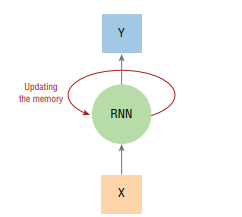
\includegraphics[width=7cm,height=5cm]{Figuras/rnn.png}
        \caption{Representación de una unidad de red neuronal recurrente.}
        \label{fig:rnncell}
    \end{center}
\end{figure}

Las unidades RNN se describen como unidades recurrentes porque el tipo de dependencia del valor actual del evento anterior es recurrente y se puede considerar como varias copias del mismo nodo, cada una de las cuales transmite un mensaje recurrente a un sucesor. Visualicemos esta relación recursiva en la Figura \ref{fig:rnnarq} \cite{francesca-lazzeri}.

\begin{figure}[H]
    \begin{center}
        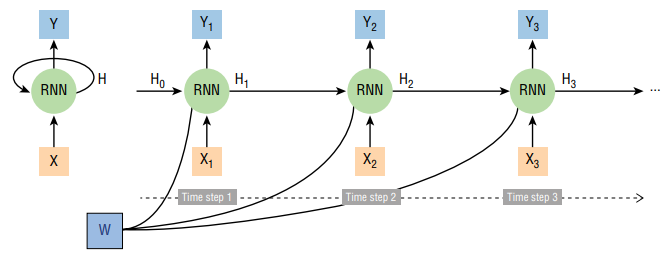
\includegraphics[width=12cm,height=5cm]{Figuras/arquitecturaRnn.png}
        \caption{Arquitectura de red neuronal recurrente.}
        \label{fig:rnnarq}
    \end{center}
\end{figure}

Las Redes Neuronales Recurrentes (RNN) se caracterizan por tener un estado oculto interno (H), el cual permite que la información se transmita entre nodos organizados en secuencias. Este estado combina datos del input actual (X) y entradas previas, y pasa por una activación tanh, que regula los valores entre -1 y 1 \cite{francesca-lazzeri} referencia. 

Las RNN utilizan un conjunto de pesos compartidos (W) para los inputs, el estado oculto previo y el output actual (Y), que se ajustan mediante el proceso de entrenamiento con optimización por descenso de gradiente. Este método actualiza los pesos calculando la función de pérdida y su derivada respecto a los pesos, moviéndose en dirección negativa del gradiente para minimizar la función de pérdida \cite{francesca-lazzeri}.

La literatura clasifica a las RNNs como \textit{Turing Complete}, lo que significa que dada la suficiente cantidad de datos y recursos computacionales, ellas simulan cualquier algoritmo de aprendizaje \cite{libro-charu}. Sin embargo, alcanzar esta meta puede ser poco realista en problemas del mundo real. Las RNNs también sufren de problemas tales como desvanecimiento y explosión de gradientes. Para superar estos problemas, se han diseñado otras redes recurrentes que incluyen a Long Short Term Memory (LSTM) y Gated Recurrent Unit (GRU).

Las RNNs y sus variantes han sido usadas en el contexto de varias aplicaciones como aprendizaje de secuencia a secuencia, descripción o subtitulado de imágenes, traducción y análisis de sentimientos \cite{libro-charu}. El procesamiento de datos de texto constituye uno de los casos de uso más comunes de RNN \cite{libro-charu}.

Tambien es importante mencionar que las RNNs se presentan como una opción natural para el pronóstico en series temporales \cite{libro-charu}. En series temporales del mundo real, el problema de aprender el próximo elemento es equivalente al análisis de Autorregresión.
Sin embargo, una RNN puede aprender modelos más complejos que aquellos obtenidos
con el modelado tradicional de series temporales \cite{libro-charu}.

Con las RNNs es común el uso de dos o tres capas en aplicaciones prácticas. De tal forma a poder usar una mayor cantidad de capas, es importante acceder a más datos de entrenamiento, de tal forma a evitar el sobre-entrenamiento \cite{libro-charu}.

\subsection{Redes Neuronales Recurrentes LSTM (Long Short-Term Memory)}

Las redes neuronales recurrentes del tipo LSTM (\textit{Long Short-Term Memory}) introdujeron la capacidad de aprender mejor las dependencias a largo plazo, una característica crucial en diversas aplicaciones de las RNN, como el modelado de series temporales. A diferencia de las RNN tradicionales, las LSTM cuentan con una estructura interna diseñada para mitigar el problema del desvanecimiento del gradiente, lo que las hace más efectivas para manejar secuencias con relaciones temporales prolongadas.

Cada unidad LSTM incluye un \textit{estado interno} y un mecanismo adicional denominado \textit{estado de celda}, que actúa como una memoria a largo plazo. Este estado de celda se regula mediante tres compuertas específicas, cada una implementada por pequeñas redes neuronales internas. Estas compuertas controlan el flujo de información dentro de la celda y son esenciales para su funcionamiento.

\subsubsection{Compuerta de Olvido}

La \textit{compuerta de olvido} determina qué información debe descartarse del estado de celda anterior. Su comportamiento se define mediante la siguiente ecuación:

\begin{equation}
    f_t = \sigma(W_f \cdot [h_{t-1}, x_t] + b_f)
\end{equation}

Donde:  
\begin{itemize}
    \item \(f_t\) es el vector de activación de la compuerta de olvido en el instante \(t\).  
    \item \(\sigma\) es la función sigmoide, que produce valores entre 0 y 1, indicando cuánto "olvidar".  
    \item \(W_f\) y \(b_f\) son los pesos y sesgos de la compuerta, aprendidos durante el entrenamiento.  
    \item \(h_{t-1}\) es el estado oculto anterior.  
    \item \(x_t\) es la entrada en el tiempo actual.
\end{itemize}

\subsubsection{Compuerta de Entrada}

La \textit{compuerta de entrada} decide qué nueva información debe incorporarse al estado de celda. Este proceso se realiza en dos pasos: calcular un vector de actualización y decidir qué información actualizar. Las ecuaciones relevantes son:

\begin{equation}
    i_t = \sigma(W_i \cdot [h_{t-1}, x_t] + b_i)
\end{equation}

\begin{equation}
    \tilde{C}_t = \tanh(W_C \cdot [h_{t-1}, x_t] + b_C)
\end{equation}

\begin{equation}
    C_t = f_t \cdot C_{t-1} + i_t \cdot \tilde{C}_t
\end{equation}

Donde:  
\begin{itemize}
    \item \(i_t\) es el vector de activación de la compuerta de entrada.  
    \item \(\tilde{C}_t\) representa los valores candidatos para actualizar el estado de celda.  
    \item \(C_t\) es el nuevo estado de celda, resultado de combinar lo que se mantiene (\(f_t \cdot C_{t-1}\)) y lo que se actualiza (\(i_t \cdot \tilde{C}_t\)).
\end{itemize}

\subsubsection{Compuerta de Salida}

La \textit{compuerta de salida} actualiza el \textit{estado oculto} y pasa la información a la siguiente unidad. Sus ecuaciones son:

\begin{equation}
    o_t = \sigma(W_o \cdot [h_{t-1}, x_t] + b_o)
\end{equation}

\begin{equation}
    h_t = o_t \cdot \tanh(C_t)
\end{equation}

Donde:  
\begin{itemize}
    \item \(o_t\) es el vector de activación de la compuerta de salida.  
    \item \(h_t\) es el estado oculto actualizado, usado para predicciones o para alimentar la siguiente celda.
\end{itemize}

El flujo de información en las LSTM se puede resumir de la siguiente manera:  
\begin{enumerate}
    \item \textbf{Decisión de olvido}: \(f_t\) regula qué información del estado anterior (\(C_{t-1}\)) debe eliminarse.  
    \item \textbf{Incorporación de nueva información}: \(i_t\) y \(\tilde{C}_t\) actualizan el estado de celda.  
    \item \textbf{Producción de salida}: \(o_t\) controla qué parte del estado de celda se refleja en el estado oculto (\(h_t\)).
\end{enumerate}

Estas ecuaciones proporcionan una base matemática que sustenta el funcionamiento de las LSTM, destacando cómo cada compuerta interactúa para gestionar las dependencias temporales en los datos.

\subsection{Redes Neuronales Recurrentes GRU (Gated Recurrent Unit)}

Las redes neuronales recurrentes del tipo GRU (\textit{Gated Recurrent Unit}) son una variante simplificada de las LSTM (\textit{Long Short-Term Memory}) introducida para reducir la complejidad computacional al mantener un desempeño competitivo en tareas de modelado de series temporales y manejo de secuencias. A diferencia de las LSTM, las GRU no poseen un estado de celda independiente; en su lugar, integran las funcionalidades del estado oculto y del estado de celda en un único vector, lo que disminuye el número de parámetros y simplifica su arquitectura.

Las GRU emplean dos compuertas principales, en lugar de tres como las LSTM: la \textbf{compuerta de actualización} y la \textbf{compuerta de reinicio}. Estas compuertas regulan el flujo de información de manera eficiente, permitiendo que el modelo aprenda tanto dependencias a corto como a largo plazo.

\subsubsection{Compuerta de Actualización}

La \textit{compuerta de actualización} controla la cantidad de información del estado oculto anterior que debe mantenerse y cuánto del nuevo estado candidato debe incorporarse al estado oculto actual. Su comportamiento se define mediante la siguiente ecuación:

\begin{equation}
    z_t = \sigma(W_z \cdot [h_{t-1}, x_t] + b_z)
\end{equation}

Donde:  
\begin{itemize}
    \item \(z_t\) es el vector de activación de la compuerta de actualización en el instante \(t\).  
    \item \(\sigma\) es la función sigmoide, que produce valores entre 0 y 1, indicando el grado de actualización.  
    \item \(W_z\) y \(b_z\) son los pesos y sesgos asociados a la compuerta de actualización.  
    \item \(h_{t-1}\) es el estado oculto anterior.  
    \item \(x_t\) es la entrada en el tiempo actual.
\end{itemize}

\subsubsection{Compuerta de Reinicio}

La \textit{compuerta de reinicio} decide cuánta información del estado oculto anterior debe olvidarse antes de calcular el nuevo estado candidato. Su ecuación es:

\begin{equation}
    r_t = \sigma(W_r \cdot [h_{t-1}, x_t] + b_r)
\end{equation}

Donde:  
\begin{itemize}
    \item \(r_t\) es el vector de activación de la compuerta de reinicio en el instante \(t\).  
    \item \(W_r\) y \(b_r\) son los pesos y sesgos de la compuerta de reinicio.  
\end{itemize}

\subsubsection{Estado Candidato y Estado Oculto Actualizado}

El nuevo estado candidato \(\tilde{h}_t\) se calcula considerando la entrada actual \(x_t\) y el estado oculto anterior \(h_{t-1}\), modulado por la compuerta de reinicio \(r_t\):

\begin{equation}
    \tilde{h}_t = \tanh(W_h \cdot [r_t \cdot h_{t-1}, x_t] + b_h)
\end{equation}

Finalmente, el estado oculto actualizado \(h_t\) es una interpolación controlada por la compuerta de actualización \(z_t\), combinando el estado candidato \(\tilde{h}_t\) y el estado oculto anterior \(h_{t-1}\):

\begin{equation}
    h_t = (1 - z_t) \cdot h_{t-1} + z_t \cdot \tilde{h}_t
\end{equation}

\subsubsection{Diferencias Principales entre LSTM y GRU}

\begin{itemize}
    \item \textbf{Número de compuertas}:  
        - LSTM utiliza tres compuertas: olvido, entrada y salida.  
        - GRU emplea solo dos: actualización y reinicio.  

    \item \textbf{Estado de celda}:  
        - LSTM tiene un estado de celda separado del estado oculto.  
        - GRU combina ambos estados en un único vector.  

    \item \textbf{Complejidad computacional}:  
        - GRU es más simple y requiere menos parámetros, lo que puede traducirse en un entrenamiento más rápido.  

    \item \textbf{Capacidad de modelado}:  
        - LSTM puede ser más adecuada para problemas con dependencias temporales muy largas debido a su diseño más complejo.  
        - GRU, al ser más ligera, es efectiva en tareas donde la longitud de las dependencias es más moderada.
\end{itemize}

Las GRU representan una alternativa eficiente a las LSTM, ofreciendo un balance entre simplicidad y capacidad para modelar dependencias temporales.

\section{Modelado de Series Temporales con Redes Neuronales Recurrentes (RNN)}

El modelado de series temporales ha sido tradicionalmente dominado por modelos estadísticos como ARIMA (\textit{AutoRegressive Integrated Moving Average}), ampliamente utilizados debido a su simplicidad y su capacidad para modelar relaciones lineales. Sin embargo, el desarrollo de las Redes Neuronales Recurrentes (RNN, por sus siglas en inglés) ha abierto nuevas posibilidades al permitir el aprendizaje de patrones complejos y no lineales en datos secuenciales, superando algunas de las limitaciones de los enfoques tradicionales.

El modelo ARIMA se basa en supuestos estadísticos rigurosos y es efectivo cuando los datos son estacionarios o pueden transformarse en estacionarios. Este modelo combina tres componentes principales: un término autoregresivo (AR) que modela la relación entre observaciones pasadas, un término integrado (I) que maneja la tendencia en los datos mediante diferencias sucesivas y un término de media móvil (MA) que modela el error en función de errores pasados. Aunque ARIMA es efectivo en muchos contextos, su principal limitación radica en su incapacidad para modelar relaciones no lineales y su dificultad para manejar múltiples variables de entrada simultáneamente. Además, requiere un preprocesamiento exhaustivo para asegurar la estacionariedad de los datos, lo que puede ser una tarea compleja en escenarios reales.

Las RNN están diseñadas para procesar secuencias de datos y aprender dependencias temporales. A diferencia de ARIMA, las RNN pueden modelar relaciones no lineales y manejar múltiples variables de entrada de manera simultánea, lo que las hace ideales para problemas complejos de predicción en series temporales. Consideremos el problema de predecir el nivel del río Paraguay en el puerto de Asunción utilizando datos históricos de niveles del río y precipitaciones. Un modelo ARIMA solo podría manejar una de estas variables, requiriendo un enfoque separado para combinar predicciones. En contraste, una RNN, como una LSTM o una GRU, puede integrar directamente ambos conjuntos de datos, aprendiendo relaciones complejas entre ellos. Esto permite realizar predicciones más precisas y robustas sin necesidad de descomponer el problema en múltiples etapas.

La efectividad de una RNN depende en gran medida de la configuración adecuada de sus hiperparámetros, como el número de neuronas, la tasa de aprendizaje y el tamaño de la ventana deslizante. Para abordar esta tarea, se pueden utilizar técnicas avanzadas de optimización, como la búsqueda de hiperparámetros mediante \textbf{Optuna}. Este enfoque ajusta automáticamente los hiperparámetros, minimizando una función de error predefinida, como el RMSE (\textit{Root Mean Square Error}) o el MAE (\textit{Mean Absolute Error}). Esto permite encontrar configuraciones óptimas de manera más rápida y precisa en comparación con métodos de búsqueda tradicionales como la búsqueda en cuadrícula o aleatoria.